For this problem and the next one assume that logic gates can take more than 2 inputs for inputs where they are \textbf{associative}. The reason why we require this is that some operators, such as NAND and NOR, are NOT associative and thus expressions like 
\[p \uparrow q \uparrow r\] are ambiguous.

Simplifying boolean expressions isn't all that useless! It seems to have ``applications'' in digital logic via the simplification of circuits, as discussed on circuit lecture. This problem is mostly a bunch of practice problems about this topic.

\begin{enumerate}
    \item Consider the logical expression $(r \lor ((s \lor q) \land r) ) \land (\shortsim (\shortsim (s \land q) )$.
    \begin{enumerate}
        \item Draw the circuit associated with this diagram.
        \item Simplify the logical expression above and draw an updated circuit associated with this diagram.
    \end{enumerate}
    \item Do the same thing, but for the logical expression $(a \land (\shortsim b)) \lor (a \land b)$.
    \pagebreak
    \item 
    \begin{enumerate}
    \item Okay, instead of converting a boolean formula into a circuit, convert this boolean circuit I made in mspaint to a boolean formula.
    
    \begin{figure}[ht]
        \centering
        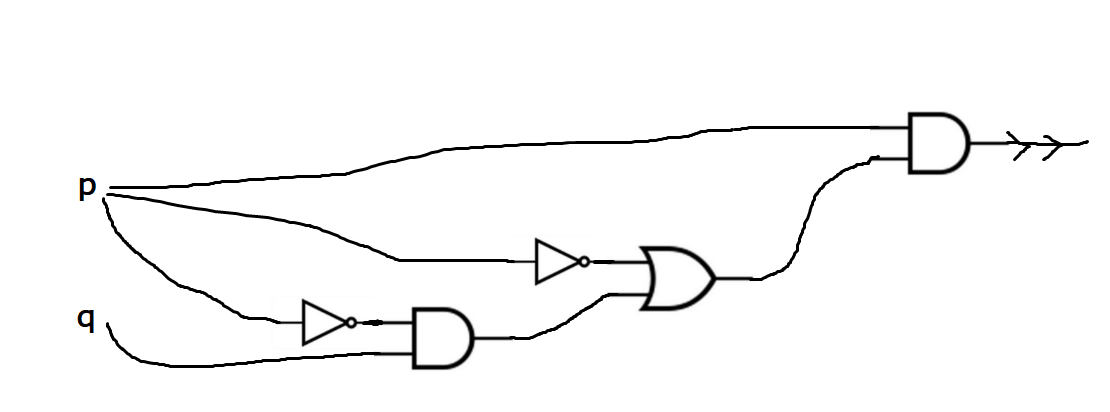
\includegraphics[width=\textwidth]{Ch2/002.png}
        \caption{Caption}
        \label{fig:my_label}
    \end{figure}
    
    \item Simplify this formula. After that, go ask around to see if there are any EE or CE majors in the room, because if you are not one of these people it is highly likely that you will not know how to draw the circuit for the simplified formula.
    \end{enumerate}
\end{enumerate}